\chapter{Introduction and Motivation}
\label{text:introduction}
Autonomous systems play an increasingly fundamental role in our society. A study by McKinsey in 2017 showed the effects of what increased automation will have on the economy. One of the keys inside of the study is that even as automation causes declines in some occupations, it will change many more, with an estimated 60 percent of occupations, of which at least 30 percent of constituent work activities will be automated.\footnote{\href{https://www.mckinsey.com/~/media/McKinsey/Featured\%20Insights/Future\%20of\%20Organizations/What\%20the\%20future\%20of\%20work\%20will\%20mean\%20for\%20jobs\%20skills\%20and\%20wages/MGI-Jobs-Lost-Jobs-Gained-Report-December-6-2017.ashx}{Jobs lost, Jobs gained: Workforce transitions in a time of automation - McKinsey Global International}} The International Federation of Robotics, an association of unilateral robotics societies and companies operating in the field, illustrated the rise of service robots in many fields, such as logistics, healthcare or agriculture, in its annual report 2019.\footnote{\href{https://ifr.org/downloads/press2018/IFR\%20World\%20Robotics\%20Presentation\%20-\%2018\%20Sept\%202019.pdf}{Annual Report 2019 - IFR}} In addition to fully autonomous robots, there the IFR also states that there is an increasing share of collaborative robots, e.g., assisting object retrieval in warehouses or cleaning in hospitals.

\begin{figure}[!ht]
\begin{center}
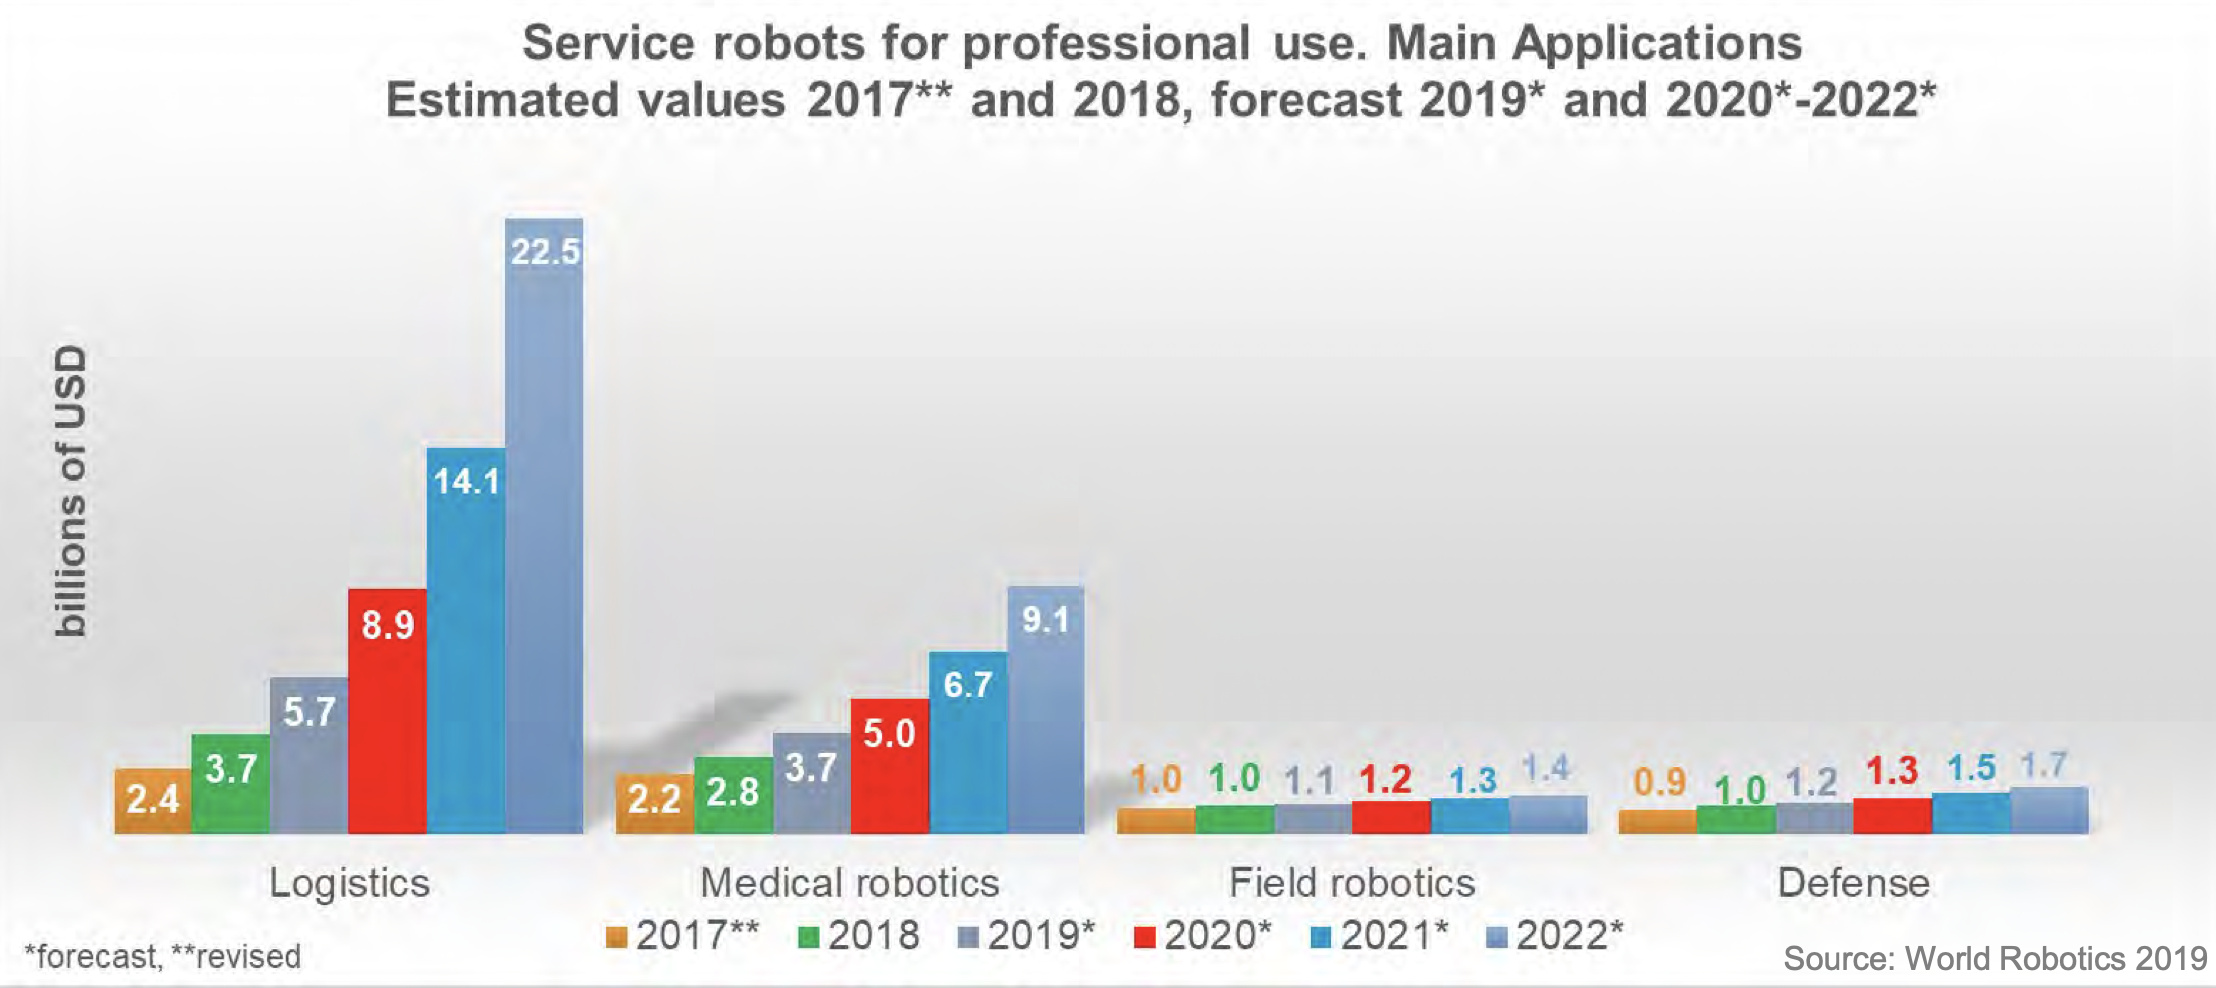
\includegraphics[width=\imgwidth]{images/service_robotics.png}
\captionof{figure}{Estimated global revenue of service robots by professional use from 2017 until 2020}
\label{img:service_robotics}
\end{center}
\end{figure}

A blog article published by the Management Review of MIT's Sloan School stated that this development might be vastly accelerated due to the societal effects of COVID-19.\footnote{\href{https://sloanreview.mit.edu/article/ai-robots-and-ethics-in-the-age-of-covid-19/}{AI, Robots, and Ethics in the Age of COVID-19 - MIT Sloan Management Review}} A perfect example of this development can be observed in the Bishan-Ang Mo Kio Park in Singapore. A robot dog, "Spot", is patrolling to monitor social distancing measures. While in the example the robot still is piloted by a human controller, in the future these systems should work entirely autonomously.\footnote{\href{http://www.straitstimes.com/singapore/meet-spot-the-safe-distancing-robot-on-trial-in-bishan-amk-park}{Meet Spot, the safe distancing robot on trial in Bishan-AMK Park - The Straits Times}}

\begin{figure}[!ht]
\begin{center}
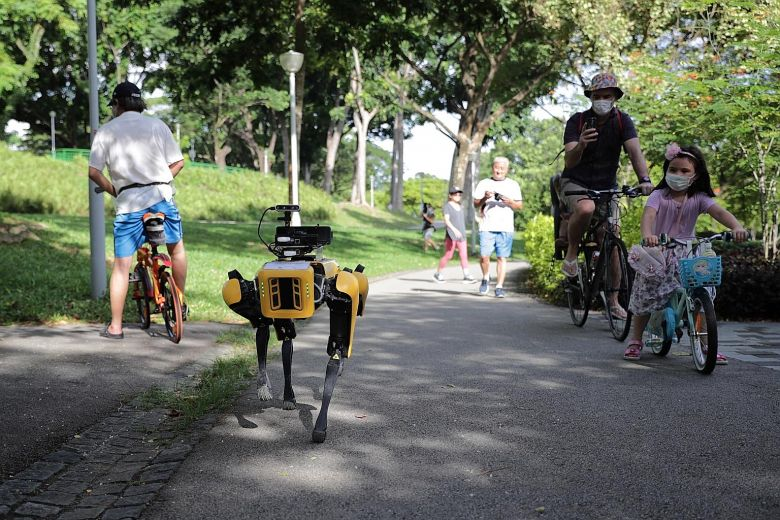
\includegraphics[width=\imgwidth]{images/spot.jpg}
\captionof{figure}{Boston Dynamics robot dog Spot patrolling in Bishan-Ang Mo Kio Park in Singapore in May 2020}
\label{img:spot_in_park}
\end{center}
\end{figure}

Summarising, robots taking part in a growing part of our social and economic life, however, efficient but more importantly safe interaction between robots and humans is crucial for its success, interactions such as walking in between them as in the example displaying in Figure \ref{img:spot_in_park}.
\newline
In interactive multi-agent scenarios, the standard control loop of perceiving the sensor input, predicting, planning, and executing the action \cite{Siegwart2011} is extended by a backward loop, due to the effects of the planned actions which have to be taken into account. Therefore after planning some future trajectory of the robot, a simulation predicts the behavior of the interacting agents, conditioned on the planned robot trajectory (comp. Figure \ref{fig:control_loop_interactive}, the idea from \cite{Romanski2019}). To guarantee interaction properties such as safety, the planner usually has to take into account the other agents' behavior. However, as the term interactive implies, this behavior depends on the planned robot trajectory. This intrinsic dependence loop is subtle and hard to approximate social norms in human interaction and a priori unknown intentions of the humans make it especially hard to deal with the interactive scenario. 

\begin{figure}
\begin{center}
\tikzstyle{block} = [draw, rectangle, minimum height=3em, minimum width=6em]
\tikzstyle{sim} = [draw, fill=cyan, rectangle, minimum height=3em, minimum width=6em]
\tikzstyle{input} = [draw, fill=orange, rectangle, minimum height=3em, minimum width=6em]
\tikzstyle{output} = [draw, fill=yellow, rectangle, minimum height=3em, minimum width=6em]
\begin{tikzpicture}[align=center, node distance=3cm,>=latex']

    \node[input, name=input](input){Sensor Input};
    \node [block, right of=input] (perception){Perception};
    \draw [->] (input) -- node {} (perception);
    \node [block, right of=perception] (prediction){Prediction};
    \draw [->] (perception) -- node[name=x] {} (prediction);
    \node [block, right of=prediction] (planning){Planning};
    \draw [->] (prediction) -- node[name=y] {} (planning);
    \node [sim, below of=y] (simulation){Simulation};
    \node [output, right of=planning] (actors){Actors};
    \draw [->] (planning) -- node[name=z] {} (actors);
    \draw [->] (z) |- (simulation);
    \draw [->] (simulation) -| (x);

\end{tikzpicture}
\captionof{figure}{Robotics control loop for interactive multi-agent scenarios}
\label{fig:control_loop_interactive}
\end{center}
\end{figure}

While humans use their "theory of mind" for reasoning about the other human's actions \cite{Gweon2013}, robots do not have this capacity (so far). Consequently, approaches that act in this highly dynamic, uncertain, and multi-modal environment try to reduce the complexity of the problem by making strong assumptions about human behavior and/or avoiding any risk. These approaches lack at least one of these properties crucial for working reliably and safely near humans: 

\begin{itemize}
\item Realistic representation of the real, complex human behavior including its multi-modal, probabilistic and highly dynamic nature
\item Guarantees on the prediction outcome which can be used to certify the safety of the system
\item Computational efficient for real-time application
\end{itemize}

When walking in crowded areas, humans use their theory of mind, giving them the capability to infer the actions of oncoming agents \cite{Ivanovic2018} \cite{Gweon2013}. To navigate through the crowd while avoiding the others as best as possible, then using the inferred information, humans leverage the inferred information and then steer towards a local minima regarding both the required travel time to reach some goal and to avoid the other pedestrian. In this way, as everyday life shows, the human way of naturally walking combines efficiency and safety. Although safety measures are not explicitly "optimized", collisions are prevented by reducing the amount of interaction, so that possibly un-safe scenarios are omitted before they can evolve instead of trying to contain safety within the interaction. In this work, we develop a robot planning algorithm for navigating in crowded, interactive scenarios. We leverage the notion that humans aim to minimize both the estimated travel time and the amount of interaction with others. The proposed robot planning algorithm depends on a "theory-of-mind" like model for prediction how agents may behave in the future.

\section{Goals}
\label{text:introduction/goals}
The goals of this work are:
\begin{itemize}
\item To design an interaction-aware planner: the robot needs to account for the responses of other agents and select plans that interferes least with others. This is important for settings where disruptions can lead to a lot of harm, such as robots operating in a hospitals, or in the example described beforehand of robots monitoring a park.
\item To provide safety assurance for the robot: the robot needs to acheive its goal safely and in a timely fashion. The prediction model may be inaccurate, or the planner does not properly account for rare yet catastrophic events. As such, there needs to be an additional layer of safety that ensures the robot remains safe regardless of the limitations of the model and/or planner.
\item To develop a real-time planning algorithm (~10Hz): in human-robot interactions, the interaction evolves rapidly and the robot needs to be able to replan sufficiently fast enough to react to rapid changes to the environment.
\end{itemize}
\section{Outline of Work}
\label{text:introduction/outline}
This thesis contains five parts. Chapter \ref{text:introduction} motivates this work, provides insights into the challenges and possible applications, defines its goals, and gives a brief overview of the solution developed within the thesis. Chapter \ref{text:related} introduces the reader into related work in the areas of the pedestrian prediction model, controls \& decision-making algorithms focussing on the interaction between robots and humans, types of trajectory optimization algorithms, and scientific notions of safety. Chapter \ref{text:approach} deep dives into the algorithm developed within this work, starting with a more detailed summary and continuing with a detailed description and explanation of each of its parts. Chapter \ref{text:experiments} validates the approach by presenting experimental results for different settings and scenarios, measuring its performance on baselines, and discussing the results. Finally, chapter \ref{text:conclusion} concludes the work and gives an outlook for future research directions.

\section{Statement of Contributions}
\label{text:introduction/contributions}
This thesis presents a trajectory optimization formulation for reliable, safe and un-disturbing navigation among pedestrians, while exploiting multi-modal and probabilistic behavior predictions.
\newline\newline
The contributions of the thesis are:

\begin{itemize}
\item Demonstrating the potentials of tightly-integrating deep data-driven, generative models in trajectory optimization, at the example of the Trajectron \cite{Ivanovic2018}\cite{Salzmann2020}. Therefore, we firstly evince the feasibility of combining such a model for online optimization, secondly expound an algorithm design that leverages the models internal knowledge representation and thirdly, we formulate an objective function design that exploits the probabilistic, multi-modal and long-horizon output of the generative model effectively and without further simplification by leveraging prior work in loss functions for training data-driven models.  
\item Using this techniques, we present a trajectory optimization formulation for socially-aware navigation among pedestrians based on multi-modal and probabilistic pedestrian predictions; focussing on the disturbance the robot's trajectory will introduce on the pedestrians as well as provable safety. In particular, a new way of pedestrian-centric trajectory optimization is introduced, explicitly targeting a socially minimally interventional way of interaction between robot and humans. For augmenting the range pedestrian prediction models, that can be combined with the presented formulation, an algorithm for transforming deterministic and short-horizon models into generative trajectory prediction models is provided.
\item Results in free-space planar simulation demonstrate the approach and benchmark it against other state-of-the-art solutions tackling socially-aware navigation.
\end{itemize}
